% Figure: Elder Parameter Space Hierarchy
% Visualizes the three-level structure with complex-valued parameters

\begin{figure}[ht]
\centering
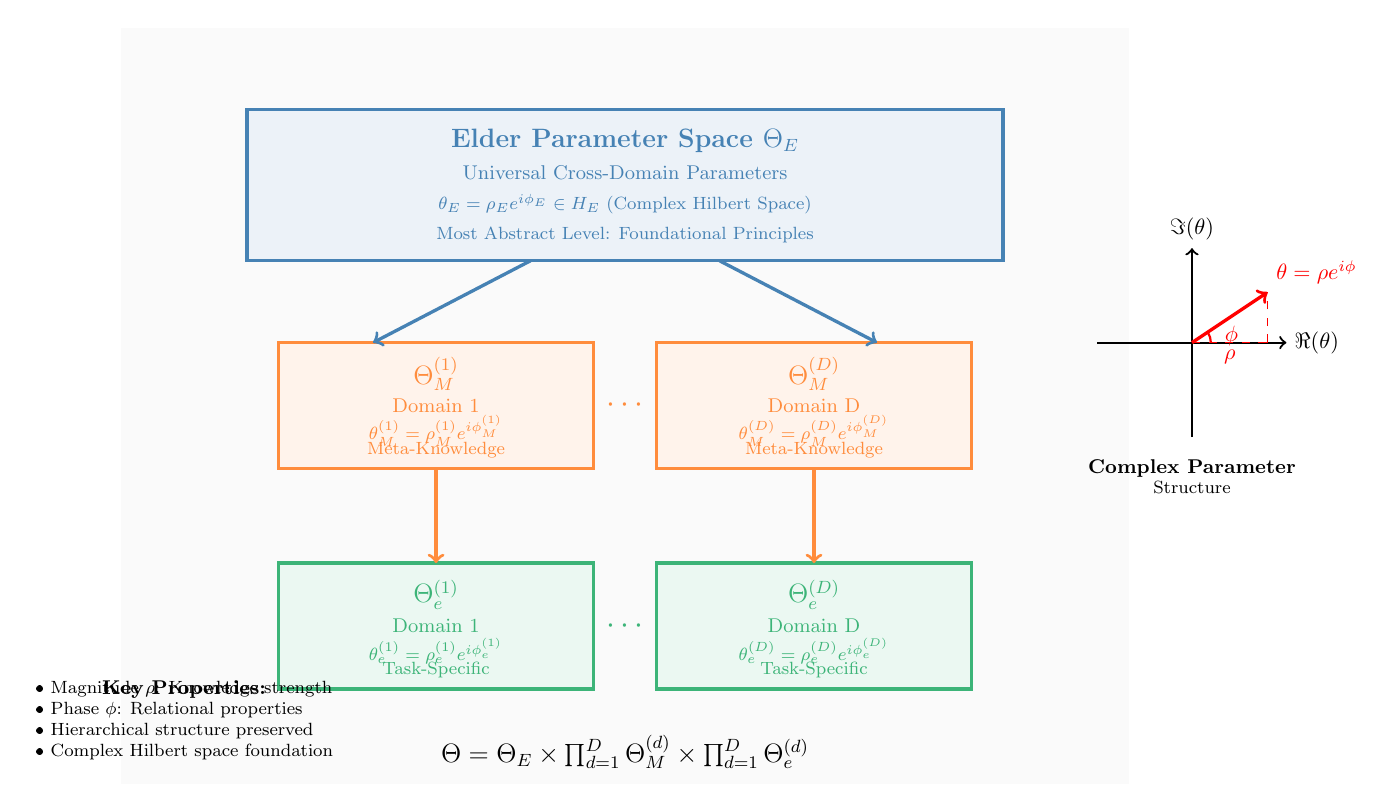
\begin{tikzpicture}[scale=0.8, every node/.style={transform shape}]

% Define colors matching Elder theme
\definecolor{ElderBlue}{RGB}{70, 130, 180}
\definecolor{MentorOrange}{RGB}{255, 140, 60}
\definecolor{EruditeGreen}{RGB}{60, 180, 120}
\definecolor{LightGray}{RGB}{240, 240, 240}

% Background
\fill[LightGray!30] (-8, -6) rectangle (8, 6);

% Elder Parameter Space (Top Level)
\begin{scope}[shift={(0, 3.5)}]
    \draw[ElderBlue, very thick, fill=ElderBlue!10] 
        (-6, -1.2) rectangle (6, 1.2);
    \node[ElderBlue, font=\large\bfseries] at (0, 0.7) {Elder Parameter Space $\Theta_E$};
    \node[ElderBlue, font=\small] at (0, 0.2) {Universal Cross-Domain Parameters};
    \node[ElderBlue, font=\footnotesize] at (0, -0.3) {$\theta_E = \rho_E e^{i\phi_E} \in \mathbb{H}_E$ (Complex Hilbert Space)};
    \node[ElderBlue, font=\footnotesize] at (0, -0.8) {Most Abstract Level: Foundational Principles};
\end{scope}

% Mentor Parameter Spaces (Middle Level)
\begin{scope}[shift={(-3, 0)}]
    \draw[MentorOrange, very thick, fill=MentorOrange!10] 
        (-2.5, -1) rectangle (2.5, 1);
    \node[MentorOrange, font=\large\bfseries] at (0, 0.5) {$\Theta_M^{(1)}$};
    \node[MentorOrange, font=\small] at (0, 0) {Domain 1};
    \node[MentorOrange, font=\footnotesize] at (0, -0.4) {$\theta_M^{(1)} = \rho_M^{(1)} e^{i\phi_M^{(1)}}$};
    \node[MentorOrange, font=\footnotesize] at (0, -0.7) {Meta-Knowledge};
\end{scope}

\begin{scope}[shift={(3, 0)}]
    \draw[MentorOrange, very thick, fill=MentorOrange!10] 
        (-2.5, -1) rectangle (2.5, 1);
    \node[MentorOrange, font=\large\bfseries] at (0, 0.5) {$\Theta_M^{(D)}$};
    \node[MentorOrange, font=\small] at (0, 0) {Domain D};
    \node[MentorOrange, font=\footnotesize] at (0, -0.4) {$\theta_M^{(D)} = \rho_M^{(D)} e^{i\phi_M^{(D)}}$};
    \node[MentorOrange, font=\footnotesize] at (0, -0.7) {Meta-Knowledge};
\end{scope}

% Dots indicating multiple domains
\node[MentorOrange, font=\Large] at (0, 0) {$\cdots$};

% Erudite Parameter Spaces (Bottom Level)
\begin{scope}[shift={(-3, -3.5)}]
    \draw[EruditeGreen, very thick, fill=EruditeGreen!10] 
        (-2.5, -1) rectangle (2.5, 1);
    \node[EruditeGreen, font=\large\bfseries] at (0, 0.5) {$\Theta_e^{(1)}$};
    \node[EruditeGreen, font=\small] at (0, 0) {Domain 1};
    \node[EruditeGreen, font=\footnotesize] at (0, -0.4) {$\theta_e^{(1)} = \rho_e^{(1)} e^{i\phi_e^{(1)}}$};
    \node[EruditeGreen, font=\footnotesize] at (0, -0.7) {Task-Specific};
\end{scope}

\begin{scope}[shift={(3, -3.5)}]
    \draw[EruditeGreen, very thick, fill=EruditeGreen!10] 
        (-2.5, -1) rectangle (2.5, 1);
    \node[EruditeGreen, font=\large\bfseries] at (0, 0.5) {$\Theta_e^{(D)}$};
    \node[EruditeGreen, font=\small] at (0, 0) {Domain D};
    \node[EruditeGreen, font=\footnotesize] at (0, -0.4) {$\theta_e^{(D)} = \rho_e^{(D)} e^{i\phi_e^{(D)}}$};
    \node[EruditeGreen, font=\footnotesize] at (0, -0.7) {Task-Specific};
\end{scope}

% Dots indicating multiple domains
\node[EruditeGreen, font=\Large] at (0, -3.5) {$\cdots$};

% Hierarchical arrows showing information flow
\draw[ElderBlue, very thick, ->] (-1.5, 2.3) -- (-4, 1);
\draw[ElderBlue, very thick, ->] (1.5, 2.3) -- (4, 1);
\draw[MentorOrange, very thick, ->] (-3, -1) -- (-3, -2.5);
\draw[MentorOrange, very thick, ->] (3, -1) -- (3, -2.5);

% Complex parameter visualization on the right
\begin{scope}[shift={(9, 1)}]
    % Complex plane representation
    \draw[black, thick, ->] (-1.5, 0) -- (1.5, 0) node[right] {$\Re(\theta)$};
    \draw[black, thick, ->] (0, -1.5) -- (0, 1.5) node[above] {$\Im(\theta)$};
    
    % Sample parameter vector
    \draw[red, very thick, ->] (0, 0) -- (1.2, 0.8) 
        node[above right] {$\theta = \rho e^{i\phi}$};
    
    % Magnitude and phase annotations
    \draw[red, dashed] (0, 0) -- (1.2, 0);
    \draw[red, dashed] (1.2, 0) -- (1.2, 0.8);
    \node[red, below] at (0.6, 0) {$\rho$};
    \draw[red, thick] (0.3, 0) arc (0:33:0.3);
    \node[red, right] at (0.4, 0.1) {$\phi$};
    
    \node[black, font=\small\bfseries] at (0, -2) {Complex Parameter};
    \node[black, font=\footnotesize] at (0, -2.3) {Structure};
\end{scope}

% Cartesian product notation
\node[black, font=\large] at (0, -5.5) {$\boldsymbol{\Theta} = \Theta_E \times \prod_{d=1}^D \Theta_M^{(d)} \times \prod_{d=1}^D \Theta_e^{(d)}$};

% Legend
\begin{scope}[shift={(-7, -5)}]
    \node[black, font=\small\bfseries] at (0, 0.5) {Key Properties:};
    \node[black, font=\footnotesize, align=left] at (0, 0) {
        • Magnitude $\rho$: Knowledge strength\\
        • Phase $\phi$: Relational properties\\
        • Hierarchical structure preserved\\
        • Complex Hilbert space foundation
    };
\end{scope}

\end{tikzpicture}

\caption{Elder Parameter Space Hierarchy. The three-level hierarchical structure shows Elder parameters $\Theta_E$ at the most abstract level containing universal cross-domain knowledge, Mentor parameters $\{\Theta_M^{(d)}\}_{d=1}^D$ at the intermediate level containing domain-specific meta-knowledge, and Erudite parameters $\{\Theta_e^{(d)}\}_{d=1}^D$ at the specialized level containing task-specific knowledge. Each parameter is complex-valued with magnitude $\rho$ encoding knowledge strength and phase $\phi$ encoding relational properties. The Cartesian product structure preserves parameter independence while maintaining hierarchical organization.}
\label{fig:elder_parameter_hierarchy}
\end{figure}